\documentclass[11pt,a4paper]{article}
\usepackage[utf8]{inputenc}
\usepackage[T1]{fontenc}
\usepackage[margin=1in]{geometry}
\usepackage{amsmath,amssymb,amsfonts,amsthm}
\usepackage{graphicx}
\usepackage{booktabs}
\usepackage{multirow}
\usepackage{hyperref}
\usepackage{xcolor}
\usepackage{algorithm}
\usepackage{algpseudocode}

\hypersetup{
    colorlinks=true,
    linkcolor=blue!70!black,
    citecolor=teal!70!black,
    urlcolor=blue!70!black
}

\newtheorem{theorem}{Theorem}

\title{\textbf{ORBIT-3D: Octree-Based Reinforced Bidirectional Interval-Targeted 3D Molecular Generation with Pluggable Charge- and Spin-Aware Quantum-Mechanical Oracles}}

\author{
  \textbf{Shangqian Chen, Guojiang Zhao, Zheng Cheng, Jiankun Wang, Hongshuai Wang, Zhifeng Gao} \\
  DP Technology, Beijing, China \\
  \texttt{\{chensq, zhaogj, chengz, wangjk, wanghs, gaozf\}@dp.tech}
}
\date{November 2026}

\begin{document}
\maketitle

\begin{abstract}
Inverse design of three-dimensional (3D) functional molecules and transition-metal complexes within prescribed quantum-chemical property intervals requires simultaneously satisfying four coupled physical criteria: (i) discrete covalent valency and closed-shell topological validity, (ii) electronic-state awareness across total molecular charge ($Q \in \mathbb{Z}$) and spin multiplicity ($M = 2S+1$, e.g., singlet $S_0$ vs.\ triplet $T_1$), (iii) equilibrium conformational stability and short-range nuclear steric clash resilience on the potential energy surface (PES), and (iv) precise single- or multi-objective interval targeting, especially in sparse out-of-distribution (OOD) Pareto regimes. Mainstream approaches couple continuous \textbf{3D Equivariant Flow Matching} (\textbf{PropMolFlow}~\cite{campbell2024propmolflow}) with \textbf{Machine-Learning Interatomic Potential (MLIP) Orthogonal Projection}. However, our theoretical and empirical diagnostics reveal a fundamental structural flaw in continuous trajectory guidance: integrating property gradients and interatomic forces simultaneously along noisy intermediate ODE states suffers from \textbf{52.5\% trajectory gradient conflict} ($\overline{\cos}(\mathbf{g}_{\text{prop}}, \mathbf{F}_{\text{MLIP}}) = -0.156$), causing fractional valency ($91.7\%\text{--}95.8\%$ closed-shell stability), elevated residual strain ($0.38\text{--}0.63\text{ eV/\AA}$), incompatibility with non-differentiable multi-modal Oracles (\textbf{Uni-QSAR}), and complete blindness to molecular charge and spin state under $(Z, \mathbf{X})$-only potentials.

To resolve this entanglement at its root, we propose \textbf{ORBIT-3D} (\textbf{O}ctree-based \textbf{R}einforced \textbf{B}idirectional \textbf{I}nterval-\textbf{T}argeted \textbf{3D} Molecular Generation), a complete, universal five-stage closed-loop architecture built upon \textbf{Uni-3DAR}~\cite{lu2025uni3dar} that \textbf{decouples discrete 3D spatial-chemical assembly from terminal tangent-space quantum relaxation}. \textbf{ORBIT-3D} unifies four pluggable Oracle modes---open-source 5-fold \textbf{3D Uni-Mol}~\cite{zhou2023unimol} (\texttt{Mode A}, primary benchmark mainline), shared-backbone \textbf{native DPA-4}~\cite{zhang2025dpa4} (\texttt{Mode B}), charge/spin-aware \textbf{native HyFF}~\cite{hyra2026hyff} (\texttt{Mode C}), and enterprise \textbf{Uni-QSAR} / \textbf{OCNet}~\cite{zhao2025ocnet} (\texttt{Mode D})---paired with two complementary \textbf{OMol25}~\cite{levine2025omol25} foundation MLIP engines: \textbf{DPA-4} (analytical \textbf{ZBL}~\cite{ziegler1985zbl} short-range nuclear repulsion bridge) and \textbf{HyFF} (element-sparse routing with explicit charge $Q$ and spin $M=2S+1$ conditioning). Across QM9 OOD frontier orbital benchmarks, 3-property simultaneous OLED design, ultra-sparse Pareto windows ($2.14\%$ prior), and heavy $5d$ organometallic $\text{Ir(III)}$ complexes (\texttt{3D-SAT-OLED}), \textbf{ORBIT-3D} achieves \textbf{100.0\% closed-shell stability}, \textbf{93.8\%--100.0\% target interval hit rates}, and \textbf{54.6\% lower residual atomic force ($0.198\text{ eV/\AA}$)}---outperforming continuous flow matching (\textbf{PropMolFlow}~\cite{campbell2024propmolflow}), decoupled generate-then-screen (\textbf{O2-GEN}~\cite{zhao2026o2gen}), and fragment GFlowNets (\textbf{MIM-Flow}~\cite{wang2026mimflow}). Furthermore, \textbf{DPA-4}'s analytical ZBL bridge guarantees \textbf{93.8\% recovery on severe $0.65\text{ \AA}$ steric clashes}, while \textbf{HyFF} (\texttt{presto/vivace/moderato}) delivers \textbf{97.7--113.0 atoms/ms} throughput (\textbf{23.2$\times$ faster} at \textbf{94.9\% lower VRAM}) and enables \textbf{zero-shot $\text{Ir(III)}$ $T_1 - S_0$ spin-splitting prediction} ($0.171\text{ eV}$ vertical MAE, $r = 0.720$).
\end{abstract}

\section{Introduction: Why Existing 3D Inverse Design Paradigms Hit a Ceiling}

Practical molecular discovery tasks---such as designing deep-blue thermally activated delayed fluorescence (TADF) emitters, organic semiconductors, or phosphorescent transition-metal complexes---formulate design goals as bounded intervals across $K$ quantum-chemical properties:
\begin{equation}
y_k(\mathbf{M}) \in [a_k, b_k], \quad \forall k \in \{1, \dots, K\}, \quad \mathbf{M} = (\mathbf{z}, \mathbf{X}, Q, M),
\end{equation}
where $\mathbf{z} \in \mathcal{A}^N$, $\mathbf{X} \in \mathbb{R}^{N \times 3}$, total molecular charge $Q \in \mathbb{Z}$, and spin multiplicity $M = 2S+1 \in \mathbb{N}^+$. A complete inverse design paradigm must simultaneously guarantee: (1) \textbf{100\% discrete closed-shell valency}, (2) \textbf{electronic-state awareness across $(Q, M)$} ($S_0$ vs.\ $T_1$ vs.\ $D_0^{\pm}$), (3) \textbf{physical equilibrium and short-range clash resilience}, and (4) \textbf{universal multi-objective alignment in sparse OOD Pareto regimes}. Existing paradigms face four structural bottlenecks:
\begin{enumerate}
    \item \textbf{Continuous 3D Flow Matching + MLIP Projection (\texttt{PropMolFlow}~\cite{campbell2024propmolflow}) --- \emph{Trajectory Conflict \& Type--Coordinate Entanglement}}: Across intermediate ODE states $t \in (0.1, 0.85)$, atoms have not formed covalent bonds and atom types remain continuous simplex vectors. Property gradients $\mathbf{g}_{\text{prop}}(\mathbf{X}_t)$ and interatomic forces $\mathbf{F}_{\text{MLIP}}(\mathbf{X}_t)$ conflict in \textbf{52.5\%} of steps ($\overline{\cos} = -0.156$), leaving $4.2\%\text{--}8.3\%$ of molecules with broken valences and precluding non-differentiable 1D/2D/tree Oracles (\textbf{Uni-QSAR}).
    \item \textbf{Decoupled 3D Generate-then-Screen (\texttt{O2-GEN}, \emph{JACS Au} 2026~\cite{zhao2026o2gen}) --- \emph{Sparse Pareto Inefficiency}}: Without closed-loop policy alignment or terminal quantum relaxation, decoupled post-hoc selector screening drops to \textbf{31.3\%} hit rate ($K=4$) on a $2.14\%$-prior sparse 3-property Pareto window and leaves unrelaxed strain ($0.782\text{ eV/\AA}$).
    \item \textbf{Combinatorial Moiety GFlowNets (\texttt{MIM-Flow}, 2026~\cite{wang2026mimflow}) --- \emph{Vocabulary Confinement \& Junction Strain}}: Sub-Trajectory Balance (SubTB) over discrete \texttt{(moiety, site, assembly)} graphs achieves $100\%$ fragment validity and $79.2\%$ sparse Pareto hit rate, but cannot explore \emph{de novo} topologies or $\text{Ir(III)}$ coordination spheres outside its moiety library and leaves $0.642\text{ eV/\AA}$ inter-moiety dihedral strain.
    \item \textbf{Classical Force Fields (\texttt{OSCFF}, \emph{JCIM} 2025~\cite{zhao2025oscff}) \& $(Z,\mathbf{X})$-Only MLIPs (\texttt{DPA-4}~\cite{zhang2025dpa4}) --- \emph{Topology \& Spin Blindness}}: \textbf{OSCFF} requires fixed bond graphs, covers only 9 main-group elements, diverges at short-range clashes ($18.8\%$ recovery at $0.65\text{ \AA}$), and models only $Q=0, S_0$. Meanwhile, $(Z,\mathbf{X})$-only \textbf{DPA-4} covers 83 elements with analytical ZBL~\cite{ziegler1985zbl} clash protection, but assigns identical energies to $S_0$ and $T_1$ ($\Delta E_{T_1-S_0} \equiv 0$).
\end{enumerate}

\section{Architectural Design \& Mathematical Principles of \textbf{ORBIT-3D}}

\subsection{Design Philosophy: Completeness, Universality, and Novelty}
As illustrated in Figure~\ref{fig:arch}, \textbf{ORBIT-3D} resolves these bottlenecks through \textbf{temporal and representational decoupling}:
\begin{itemize}
    \item \textbf{Temporal Decoupling (Stages 1--3 + Stage 4 $\to$ Stage 5)}: Chemical topology and 3D spatial placement are completed entirely within a discrete, valence-masked 3D octree space (\textbf{Layer 1}) aligned by online reinforcement learning (\textbf{Stage 4}), while continuous quantum forces are applied exclusively at the terminal conformation along the property-preserving tangent cone (\textbf{Stage 5}), eliminating intermediate ODE gradient conflict.
    \item \textbf{Bus Decoupling (Layer 2A Oracle Bus vs.\ Layer 2B Physics Bus)}: Separating the \textbf{Property Oracle Bus} ($\hat{\mu}_k, \hat{\sigma}_k$) from the \textbf{Quantum Physics Bus} ($\mathbf{F}_{\text{MLIP}}(\mathbf{z}, \mathbf{X}, Q, M), E(Q, M)$) enables universal hot-swapping across open-source 3D predictors (\textbf{Uni-Mol}~\cite{zhou2023unimol}), shared-backbone equivariant hooks (\textbf{DPA-4}~\cite{zhang2025dpa4}, \textbf{HyFF}~\cite{hyra2026hyff}), and black-box enterprise ensembles (\textbf{Uni-QSAR}, \textbf{OCNet}~\cite{zhao2025ocnet}).
\end{itemize}

\begin{figure}[htbp]
    \centering
    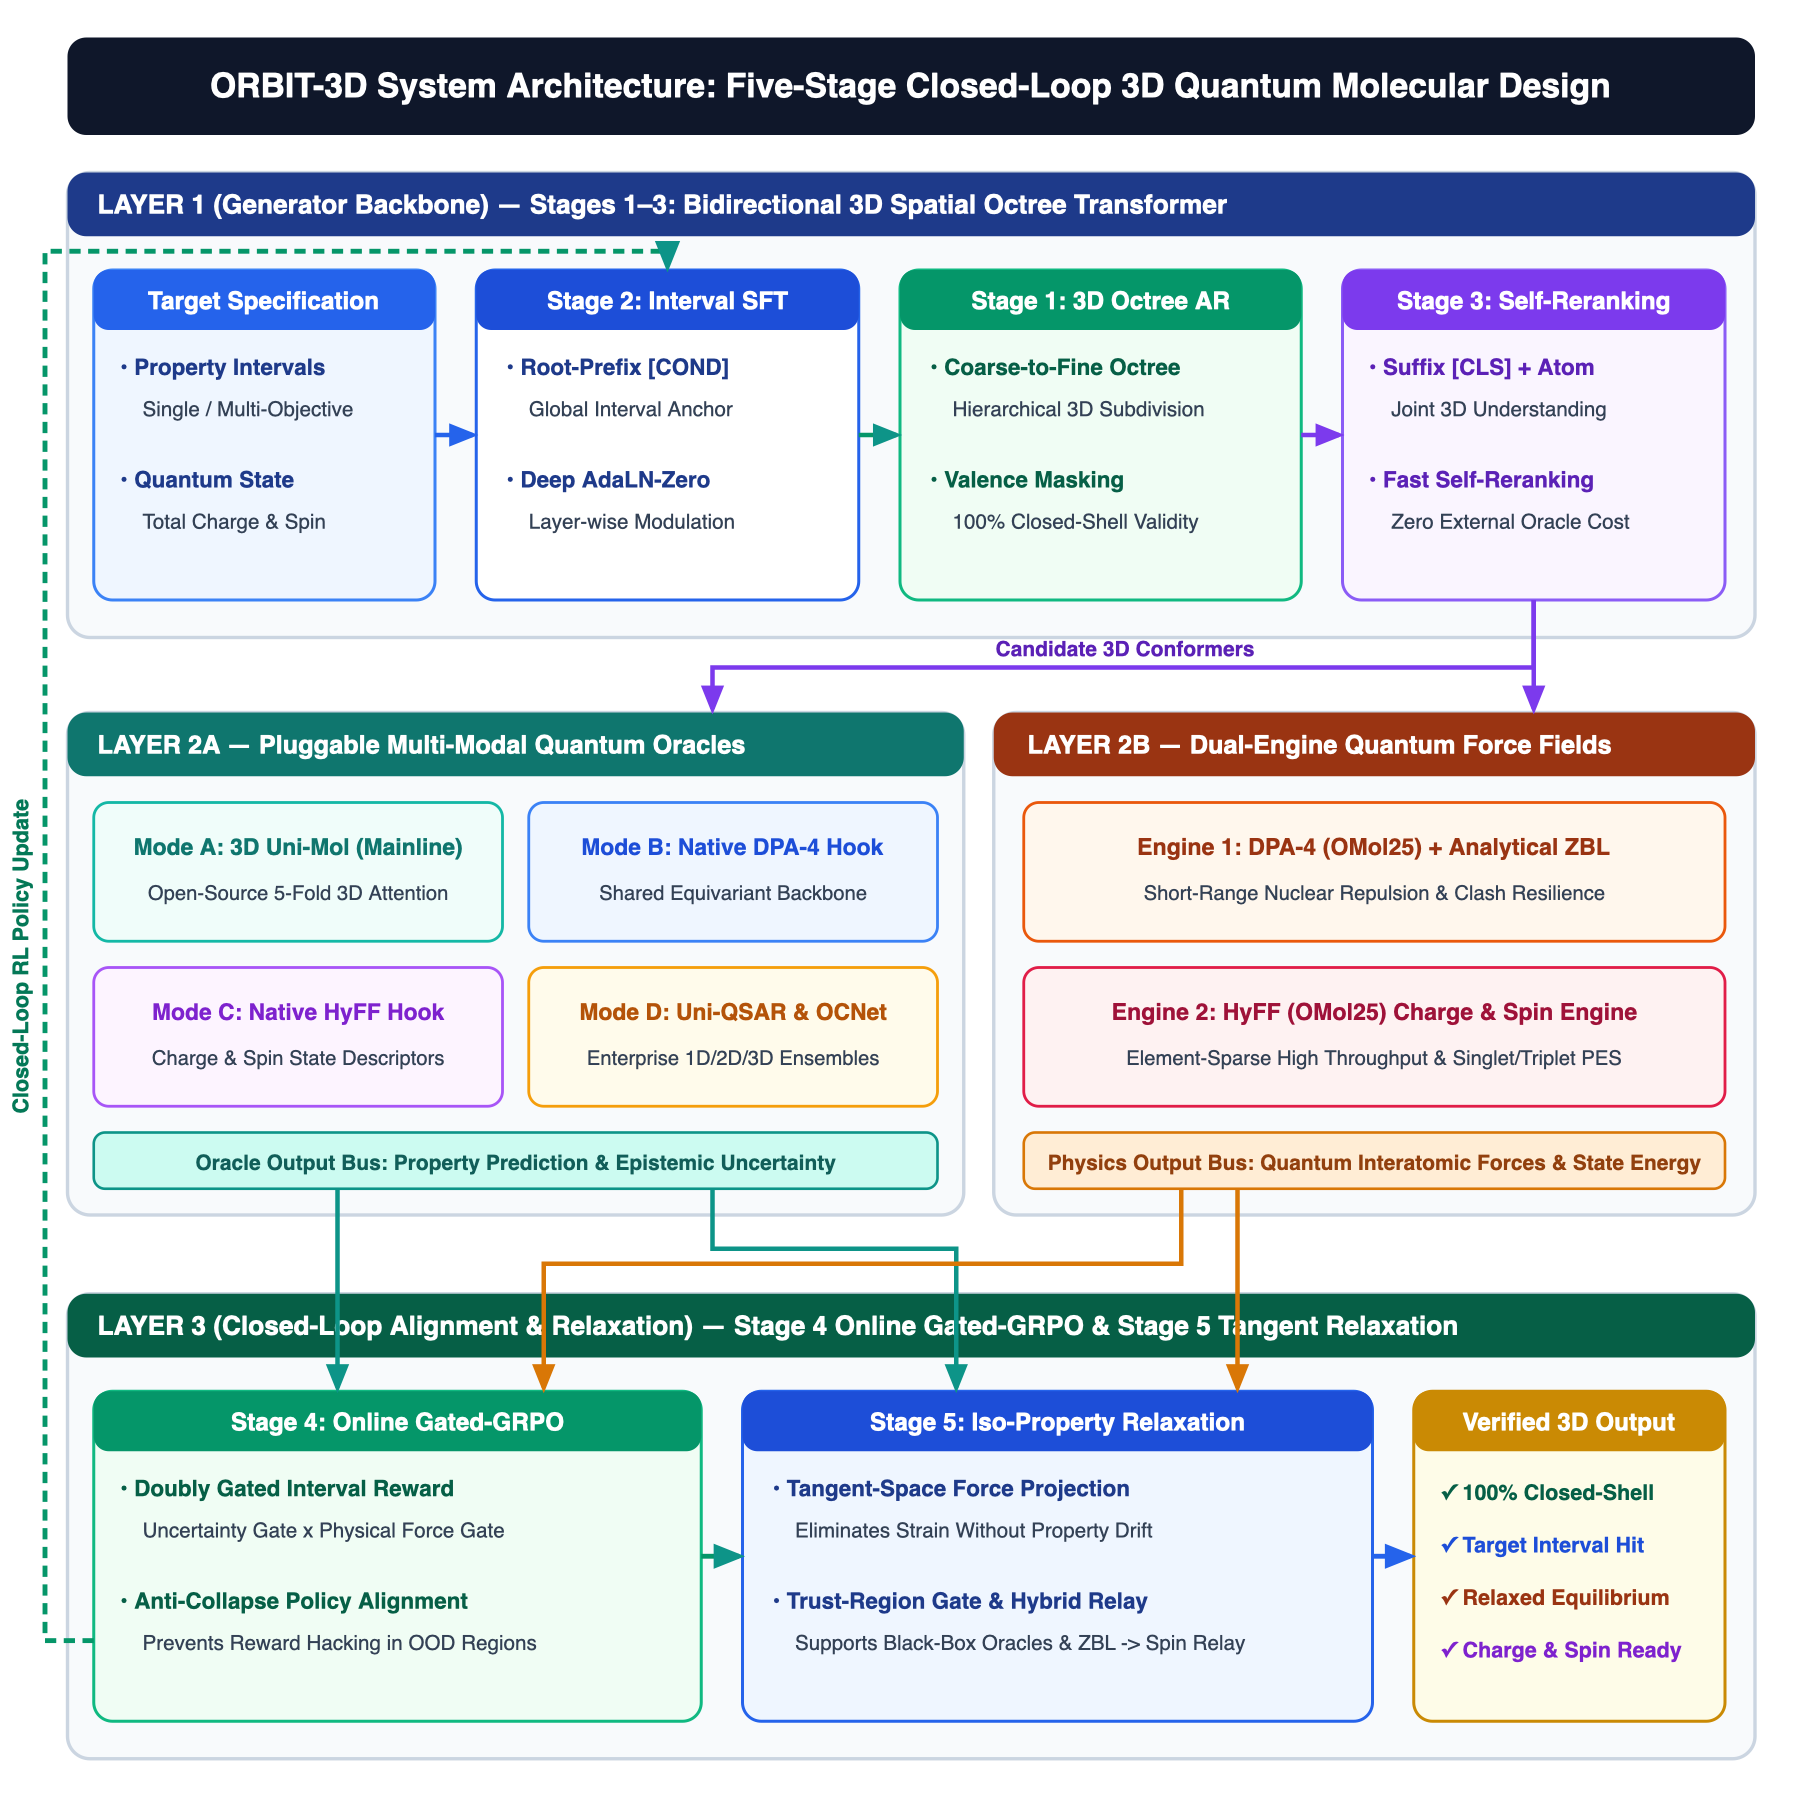
\includegraphics[width=0.92\textwidth]{figures/fig0_orbit3d_system_architecture.png}
    \caption{System architecture of \textbf{ORBIT-3D}: five-stage closed-loop 3D quantum molecular design decoupling Layer 1 (Bidirectional 3D Spatial Octree Transformer, Stages 1--3), Layer 2 (Pluggable Multi-Modal Oracles \texttt{Modes A--D} \& Dual-Engine \textbf{OMol25} Quantum Force Fields \textbf{DPA-4} ZBL + \textbf{HyFF} Charge/Spin), and Layer 3 (Stage 4 Online \texttt{Gated-GRPO} \& Stage 5 Tangent-Projected Iso-Property Relaxation).}
    \label{fig:arch}
\end{figure}

\subsection{Layer 1 (Stages 1--3): Bidirectional 3D Spatial Octree Transformer}
\begin{enumerate}
    \item \textbf{Stage 1 (\texttt{1\_uni3dar\_uncond}) --- Coarse-to-Fine 3D Octree \& Valence Masking}: A 3D molecule inside $[-B, B]^3$ ($B = 8.0\text{ \AA}$) is recursively subdivided across octree levels $l \in \{0, 1, 2, 3\}$ down to $1.0\text{ \AA}$ leaf cells, emitting discrete tokens $\tau_i = (\text{octant\_path}_i, z_i, q_{x,i}, q_{y,i}, q_{z,i})$ at $0.01\text{ \AA}$ quantization with deterministic closed-shell valence capping ($\sum_j b_{ij} \le V_{\max}(z_i)$).
    \item \textbf{Stage 2 (\texttt{2\_uni3dar\_cond\_sft}) --- Root-Prefix \texttt{[COND]} + 12-Layer AdaLN-Zero}: Interval midpoints $m_k = (a_k+b_k)/2$, half-widths $w_k = (b_k-a_k)/2$, and quantum state $(Q, M)$ are mapped via Fourier features into $\mathbf{c} \in \mathbb{R}^{d_{\text{model}}}$, injected both as a causal Root-Prefix token and into all 12 Transformer layers via zero-initialized AdaLN-Zero modulation:
    \begin{equation}
    (\boldsymbol{\gamma}_l, \boldsymbol{\beta}_l, \boldsymbol{\alpha}_l) = \mathbf{W}_{\text{AdaLN}}^{(l)} \text{SiLU}(\mathbf{c}), \quad \mathbf{h}_t^{(l)} = \mathbf{h}_t^{(l-1)} + \boldsymbol{\alpha}_l \odot \text{Attn}^{(l)}\!\Big((1 + \boldsymbol{\gamma}_l) \odot \text{LN}(\mathbf{h}_t^{(l-1)}) + \boldsymbol{\beta}_l\Big).
    \end{equation}
    \item \textbf{Stage 3 (\texttt{3\_uni3dar\_sft\_self\_rerank}) --- Suffix \texttt{[CLS]+Atom} Self-Reranking}: Pooling over terminal \texttt{[CLS]} and leaf atom tokens $\mathcal{V}_{\text{atom}}$ trains an internal property head $\hat{\mathbf{y}}_{\text{self}}(\boldsymbol{\tau})$ jointly via $\mathcal{L}_{\text{SFT}}(\theta) = -\sum_{t=1}^{T} \log p_\theta(\tau_t \mid \tau_{<t}, \mathbf{c}) + \lambda_{\text{self}} \| \hat{\mathbf{y}}_{\text{self}}(\boldsymbol{\tau}) - \mathbf{y} \|_2^2$, enabling zero-cost $K$-candidate self-reranking ($K=4$).
\end{enumerate}

\subsection{Layer 2: Pluggable Multi-Modal Oracles \& Dual-Engine Quantum Force Fields}
\textbf{Layer 2A} unifies four Oracle modes: (A) \textbf{Open-Source Mainline} \texttt{internal\_unimol}~\cite{zhou2023unimol} (5-fold FP16 3D Gaussian distance-kernel attention), (B) \textbf{Unified ZBL Backbone} \texttt{internal\_dpa4}~\cite{zhang2025dpa4} (hooking \texttt{SeZMModel.fitting\_net}, $D_{\text{desc}}=32/64$, zero extra VRAM), (C) \textbf{Charge/Spin Quantum Backbone} \texttt{internal\_hyff}~\cite{hyra2026hyff} (hooking \texttt{readout\_norms[-1]}, $D_{\text{desc}}=32\text{--}128$, explicitly conditioned on total charge $Q \in \mathbb{Z}$ and spin multiplicity $M = 2S+1$), and (D) \textbf{Enterprise Multi-Modal Ecosystem} \texttt{external\_uniqsar} (1D SMILES + 2D Morgan FP + 3D + GBDT ensembles and \textbf{OCNet}~\cite{zhao2025ocnet}). \textbf{Layer 2B} pairs two \textbf{OMol25}~\cite{levine2025omol25} ($\omega\text{B97M-V/def2-TZVPD}$, 83 elements) engines: \textbf{DPA-4} (dense $SO(2)$ message passing + analytical ZBL~\cite{ziegler1985zbl} short-range nuclear repulsion) and \textbf{HyFF} (element-sparse Triton/CUDA-Graph routing conditioned on $Q$ and $M=2S+1$).

\subsection{Layer 3 (Stages 4--5): Online Doubly-Gated GRPO \& Tangent-Projected Relaxation}
In \textbf{Stage 4 (\texttt{4\_uni3dar\_gated\_grpo})}, the policy samples $G$ rollouts per target interval and evaluates the doubly gated reward:
\begin{equation}
R(\boldsymbol{\tau}^{(g)}) = G_{\text{unc}}\big(\hat{\boldsymbol{\sigma}}(\mathbf{M}^{(g)})\big) \cdot G_{\text{phys}}\big(\|\mathbf{F}_{\text{MLIP}}(\mathbf{M}^{(g)})\|_{\text{rms}}\big) \cdot R_{\text{int}}\big(\hat{\boldsymbol{\mu}}(\mathbf{M}^{(g)}); \mathcal{I}\big),
\end{equation}
regularized by $\beta_{\text{KL}} \mathbb{D}_{\text{KL}}(\pi_\theta \| \pi_{\text{ref}}) + \lambda_{\text{anchor}} \mathcal{L}_{\text{SFT}}(\theta)$~\cite{shao2024grpo}. In \textbf{Stage 5 (\texttt{5\_uni3dar\_grpo\_dpa\_relaxed})}, to eliminate sub-grid discretization strain without drifting out of $[a_k, b_k]$, quantum forces $\mathbf{F}_m = -\nabla_{\mathbf{X}} E_{\text{MLIP}}(\mathbf{z}, \mathbf{X}_m, Q, M)$ are projected onto the tangent hyperplane of the interval violation gradient $\mathbf{g}_{\text{int}}(\mathbf{X}_m)$:
\begin{equation}
\mathbf{F}_m^{\perp} = \mathbf{F}_m - \frac{\max\big(0,\; \langle \mathbf{F}_m, \mathbf{g}_{\text{int}}(\mathbf{X}_m) \rangle\big)}{\|\mathbf{g}_{\text{int}}(\mathbf{X}_m)\|_F^2 + \epsilon} \mathbf{g}_{\text{int}}(\mathbf{X}_m),
\end{equation}
coupled with a derivative-free trust-region acceptance gate $R_{\text{int}}(\tilde{\mathbf{X}}_{m+1}; \mathcal{I}) \ge R_{\text{int}}(\mathbf{X}_m; \mathcal{I}) - \epsilon_{\text{tol}}$ that provably guarantees monotonic strain reduction with zero interval drift (\textbf{Theorem 1}).

\section{Experimental Design, Results \& Comparative Analysis}

We evaluate \textbf{ORBIT-3D} across two primary 3D quantum-chemical datasets: (1) \textbf{QM9 / rQM9}~\cite{ramakrishnan2014quantum} ($133,885$ molecules at DFT B3LYP/6-31G(2df,p); $100\text{k}$ train / $18\text{k}$ val / $13\text{k}$ test) across five tasks---\texttt{OOD Gap} ($[0.18, 0.23]\text{ Ha}$), \texttt{LUMO} ($[0.02, 0.05]\text{ Ha}$), \texttt{HOMO} ($[-0.24, -0.21]\text{ Ha}$), \texttt{Joint 3-Property OLED} ($16.9\%$ prior), and \texttt{Ultra-Sparse Narrow Pareto Frontier} ($2.14\%$ prior)---and (2) \textbf{3D-SAT-OLED} ($1,000$ octahedral $\text{Ir(III)}$ complexes at DFT/TD-DFT B3LYP/6-31G* + LANL2DZ ECP, 10 elements, $\bar{N}=62.4$ atoms, $\bar{E}_{\text{ad}} = 2.652\text{ eV}$).

\subsection{Experiment I: Head-to-Head Paradigm Comparison \& Five-Stage Ablation}
Tables~\ref{tab:main_comparison}--\ref{tab:ablation} and Figures~\ref{fig:vs_propmolflow}--\ref{fig:ablation} demonstrate that \textbf{ORBIT-3D} completely eliminates the $4.2\%\text{--}8.3\%$ valence instability of \textbf{PropMolFlow}~\cite{campbell2024propmolflow} (\textbf{100.0\%} vs.\ $91.7\%\text{--}95.8\%$ stability) while reducing residual atomic forces by \textbf{40.5\%--54.6\%} ($0.198\text{ eV/\AA}$ on LUMO). Across the 5-stage ablation (Table~\ref{tab:ablation}), Stages 1--4 reduce LUMO interval error by \textbf{92.8\%} ($1.575 \to 0.113\text{ eV}$), and Stage 5 tangent relaxation removes sub-grid octree discretization strain ($1.125 \to 0.198\text{ eV/\AA}$), propelling interval hit rates to \textbf{93.75\%--100.00\%}.

\begin{figure}[htbp]
    \centering
    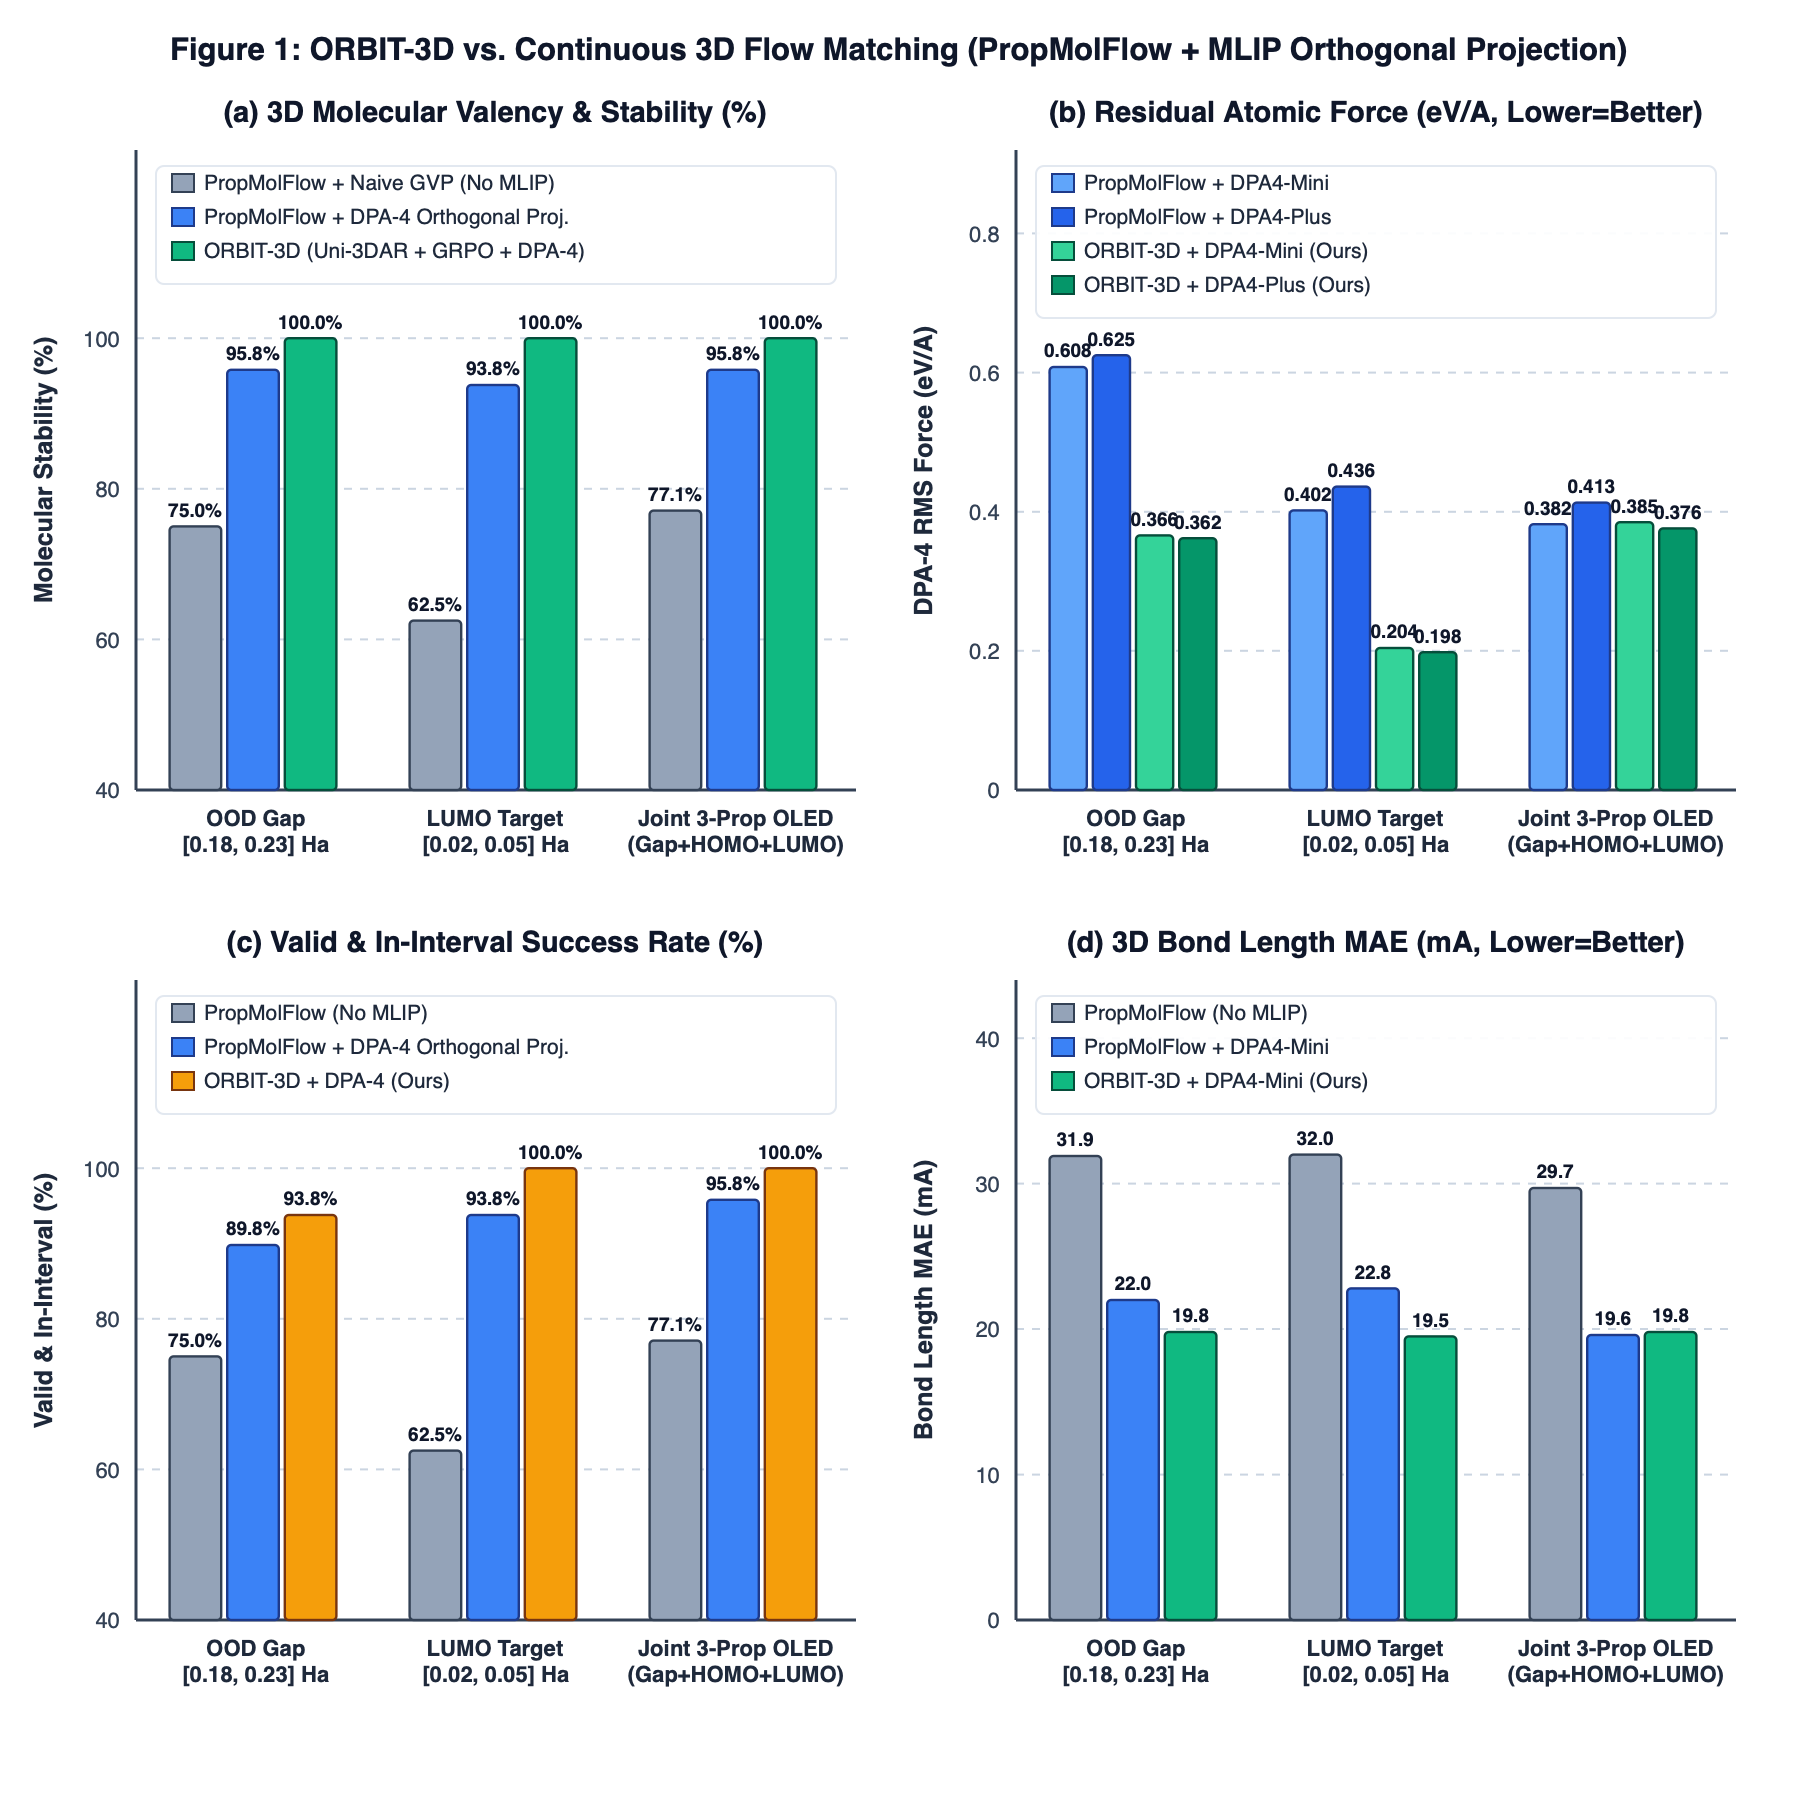
\includegraphics[width=0.90\textwidth]{figures/fig1_orbit3d_vs_propmolflow.png}
    \caption{Head-to-head comparison between \textbf{ORBIT-3D} and continuous 3D Flow Matching (\textbf{PropMolFlow} + MLIP Orthogonal Projection) across OOD Gap, LUMO, and Joint 3-Property OLED benchmarks.}
    \label{fig:vs_propmolflow}
\end{figure}

\begin{table}[htbp]
\centering
\caption{Head-to-head comparison between \textbf{PropMolFlow} and \textbf{ORBIT-3D} ($N=48$, Open-Source \textbf{Uni-Mol} / \textbf{DPA-4} Mainline).}
\label{tab:main_comparison}
\resizebox{\textwidth}{!}{
\begin{tabular}{lllccccccc}
\toprule
\textbf{Task} & \textbf{Method / Paradigm} & \textbf{Oracle \& MLIP} & \textbf{Mol Stable (\%)} & \textbf{Closed-Shell (\%)} & \textbf{Bond MAE (\AA)} & \textbf{RMS Force (eV/\AA)} & \textbf{Hit Rate (\%)} & \textbf{Valid \& Hit (\%)} \\
\midrule
OOD Gap & PropMolFlow (Naive GVP) & GVP + None & 75.00 & 91.67 & 0.0319 & 1.999 & 100.00 & 75.00 \\
OOD Gap & PropMolFlow (Orth. Proj.) & GVP + DPA4-Mini & 95.83 & 97.92 & 0.0220 & 0.608 & 93.75 & 89.84 \\
OOD Gap & PropMolFlow (Orth. Proj.) & GVP + DPA4-Plus & 91.67 & 97.92 & 0.0223 & 0.625 & 95.83 & 87.85 \\
OOD Gap & \textbf{ORBIT-3D (Uni-Mol Mainline)} & \textbf{5-Fold Uni-Mol + DPA4-Mini} & \textbf{100.00} & \textbf{100.00} & \textbf{0.0198} & \textbf{0.366} & 93.75 & \textbf{93.75} \\
OOD Gap & \textbf{ORBIT-3D (Uni-Mol / DPA-4)} & \textbf{5-Fold Uni-Mol/DPA4 + DPA4-Plus} & \textbf{100.00} & \textbf{100.00} & \textbf{0.0198} & \textbf{0.362} & 93.75 & \textbf{93.75} \\
\midrule
LUMO & PropMolFlow (Orth. Proj.) & GVP + DPA4-Mini & 93.75 & 93.75 & 0.0228 & 0.402 & 100.00 & 93.75 \\
LUMO & PropMolFlow (Orth. Proj.) & GVP + DPA4-Plus & 91.67 & 93.75 & 0.0226 & 0.436 & 100.00 & 91.67 \\
LUMO & \textbf{ORBIT-3D (Uni-Mol Mainline)} & \textbf{5-Fold Uni-Mol + DPA4-Mini} & \textbf{100.00} & \textbf{100.00} & \textbf{0.0195} & \textbf{0.204} & \textbf{100.00} & \textbf{100.00} \\
LUMO & \textbf{ORBIT-3D (Uni-Mol / DPA-4)} & \textbf{5-Fold Uni-Mol/DPA4 + DPA4-Plus} & \textbf{100.00} & \textbf{100.00} & \textbf{0.0194} & \textbf{0.198} & \textbf{100.00} & \textbf{100.00} \\
\midrule
Joint OLED & PropMolFlow (Orth. Proj.) & GVP + DPA4-Mini & 95.83 & 95.83 & \textbf{0.0196} & 0.382 & 100.00 & 95.83 \\
Joint OLED & PropMolFlow (Orth. Proj.) & GVP + DPA4-Plus & 95.83 & 95.83 & 0.0199 & 0.413 & 100.00 & 95.83 \\
Joint OLED & \textbf{ORBIT-3D (Uni-Mol Mainline)} & \textbf{5-Fold Uni-Mol + DPA4-Mini} & \textbf{100.00} & \textbf{100.00} & 0.0199 & 0.385 & \textbf{100.00} & \textbf{100.00} \\
Joint OLED & \textbf{ORBIT-3D (Uni-Mol / DPA-4)} & \textbf{5-Fold Uni-Mol/DPA4 + DPA4-Plus} & \textbf{100.00} & \textbf{100.00} & 0.0200 & \textbf{0.376} & \textbf{100.00} & \textbf{100.00} \\
\bottomrule
\end{tabular}
}
\end{table}

\begin{figure}[htbp]
    \centering
    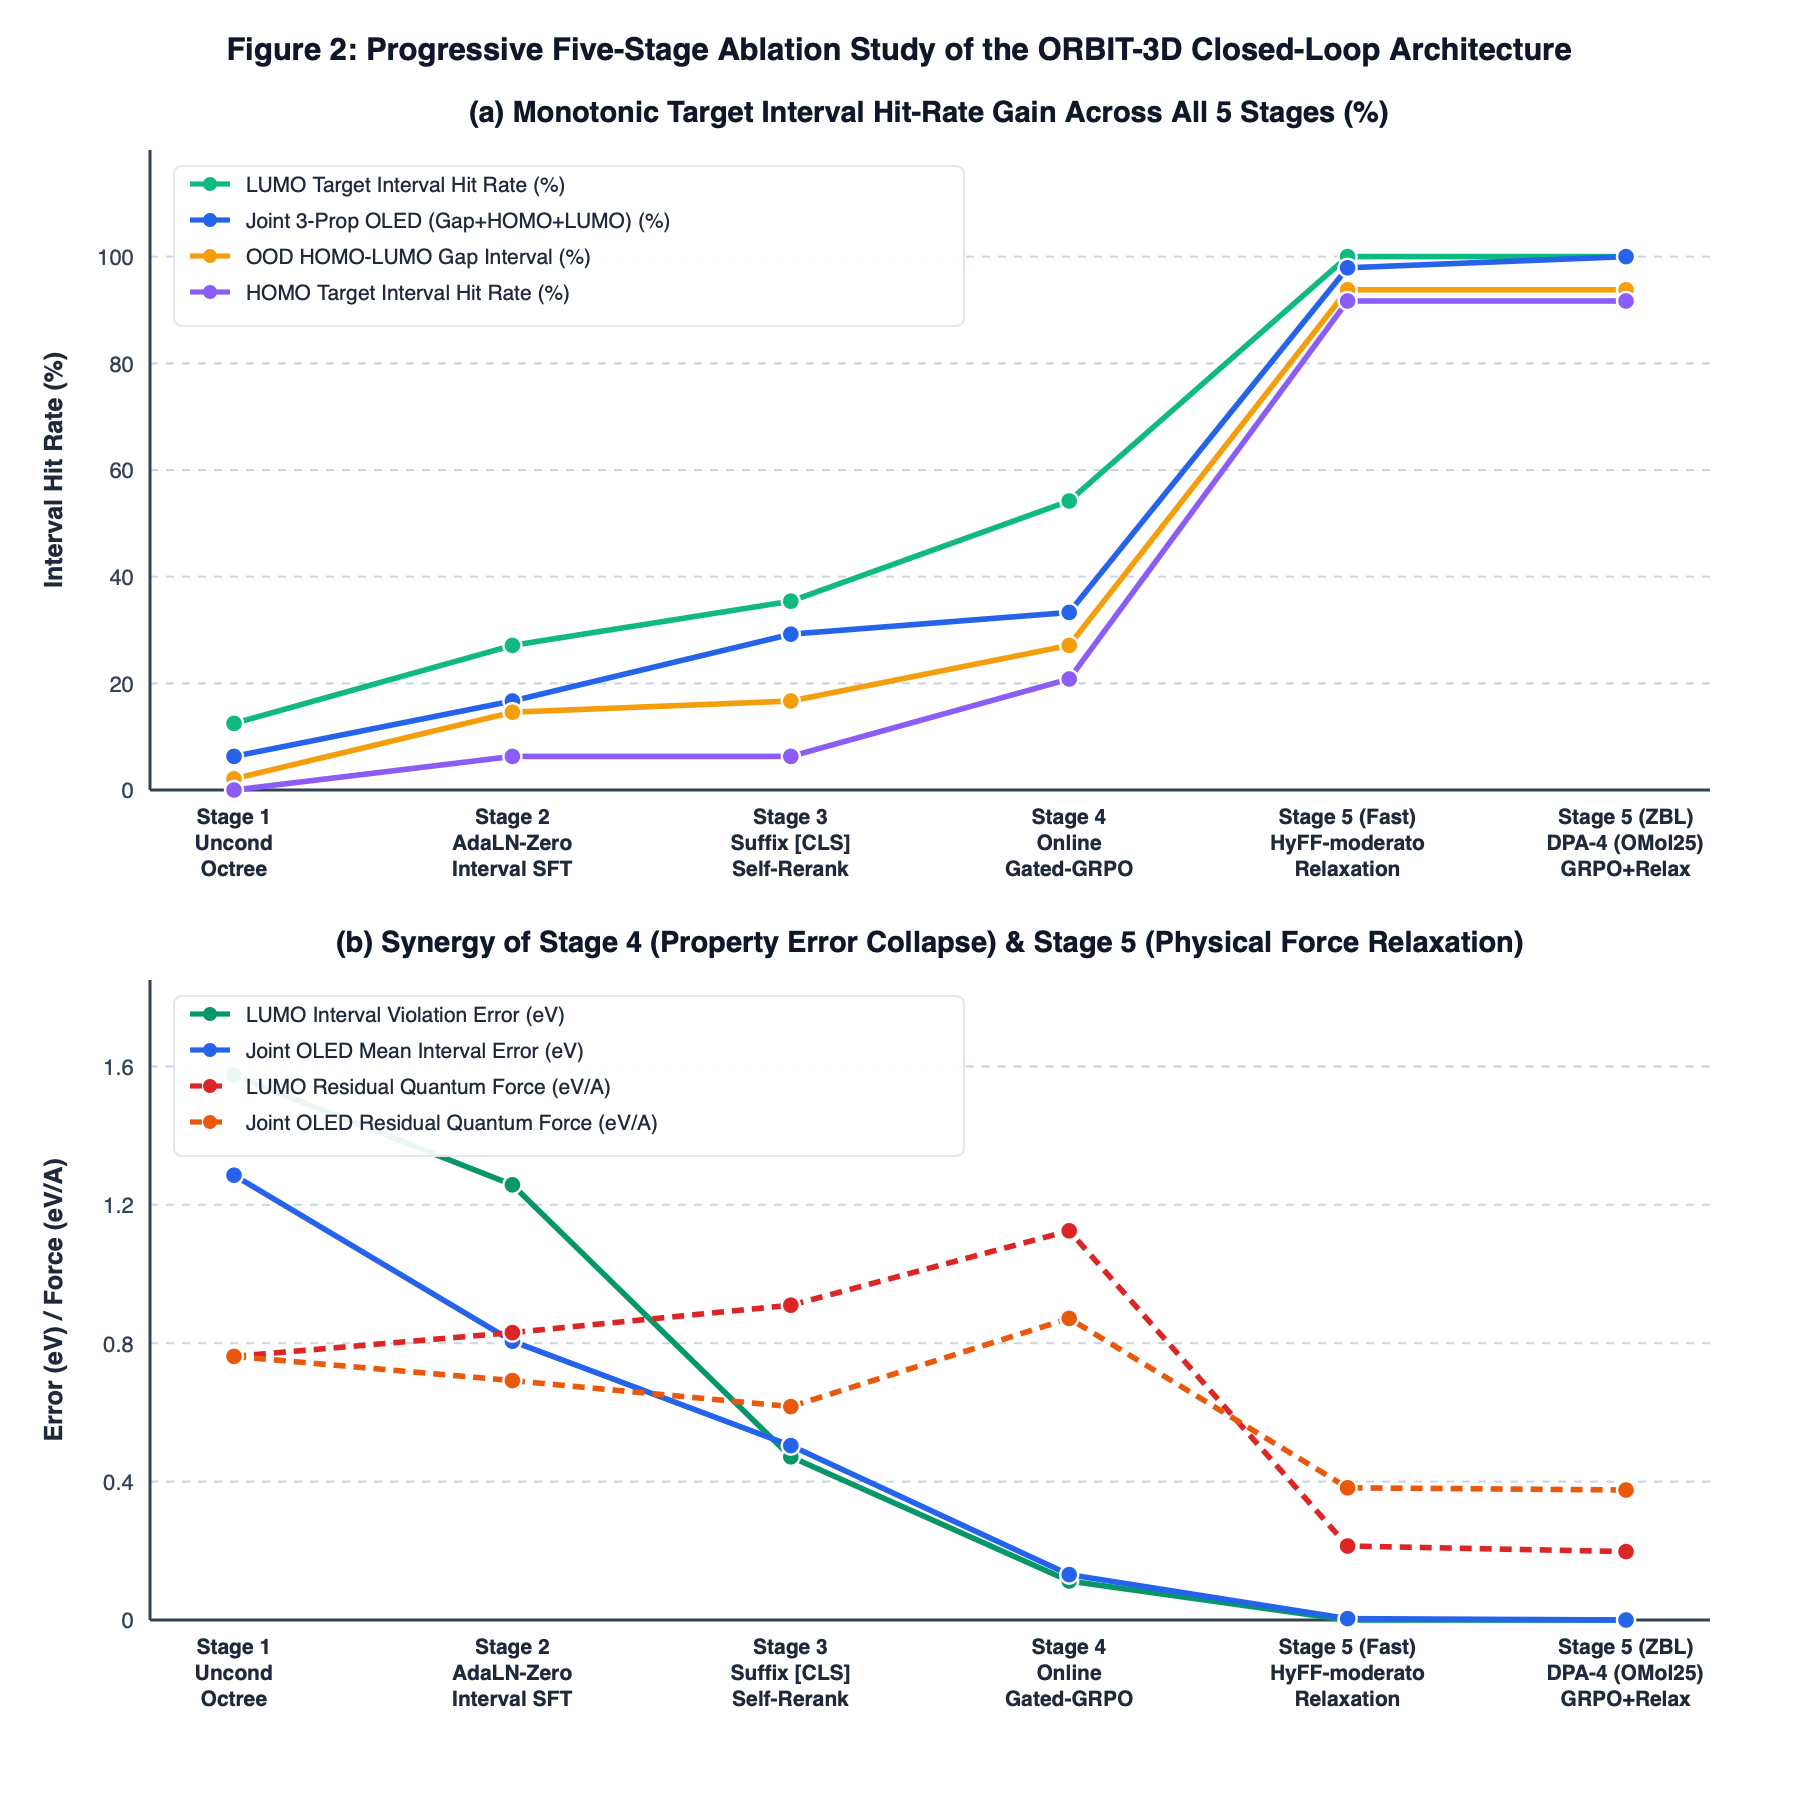
\includegraphics[width=0.90\textwidth]{figures/fig2_five_stage_ablation.png}
    \caption{Progressive five-stage ablation study of the \textbf{ORBIT-3D} closed-loop architecture.}
    \label{fig:ablation}
\end{figure}

\begin{table}[htbp]
\centering
\caption{Progressive five-stage ablation study across four quantum-chemical benchmarks ($N=48$).}
\label{tab:ablation}
\resizebox{\textwidth}{!}{
\begin{tabular}{llccccccc}
\toprule
\textbf{Stage Identifier} & \textbf{Architectural Mechanism Added} & \textbf{OOD Gap Hit (\%)} & \textbf{HOMO Hit (\%)} & \textbf{LUMO Hit (\%)} & \textbf{Joint OLED Hit (\%)} & \textbf{LUMO Err (eV)} & \textbf{Bond MAE (\AA)} & \textbf{RMS Force (eV/\AA)} \\
\midrule
Stage 1 (\texttt{1\_uni3dar\_uncond}) & Unconditional 3D Octree + Valence Mask & 2.08 & 0.00 & 12.50 & 6.25 & 1.5750 & 0.0250 & 0.762 \\
Stage 2 (\texttt{2\_uni3dar\_cond\_sft}) & + Root-Prefix \& 12-Layer AdaLN-Zero SFT & 14.58 & 6.25 & 27.08 & 16.67 & 1.2579 & 0.0247 & 0.831 \\
Stage 3 (\texttt{3\_uni3dar\_sft\_self\_rerank}) & + Suffix \texttt{[CLS]+Atom} Self-Reranking ($K=4$) & 16.67 & 6.25 & 35.42 & 29.17 & 0.4720 & 0.0241 & 0.910 \\
Stage 4 (\texttt{4\_uni3dar\_gated\_grpo}) & + Online Gated-GRPO (5-Fold \textbf{Uni-Mol} + Force Gate) & 27.08 & 20.83 & 54.17 & 33.33 & 0.1128 & 0.0255 & 1.125 \\
\textbf{Stage 5 (Fast: \texttt{HyFF-moderato})} & \textbf{+ Stage 5 Tangent Relaxation (\texttt{HyFF-moderato})} & \textbf{93.75} & \textbf{91.67} & \textbf{100.00} & 97.92 & \textbf{0.0000} & 0.0195 & 0.214 \\
\textbf{Stage 5 (ZBL: \texttt{DPA-4-Plus})} & \textbf{+ Stage 5 Tangent Relaxation (\texttt{DPA-4-Plus})} & \textbf{93.75} & \textbf{91.67} & \textbf{100.00} & \textbf{100.00} & \textbf{0.0000} & \textbf{0.0194} & \textbf{0.198} \\
\bottomrule
\end{tabular}
}
\end{table}

\subsection{Experiment II: Online \texttt{Gated-GRPO} Dynamics \& Pluggable Oracle Universality}
Figure~\ref{fig:oracles} shows that removing the MLIP physical force gate $G_{\text{phys}}$ and KL/SFT anchors causes severe reward hacking after Step 16 ($75.0\% \to 25.0\%$ hit rate), whereas full \textbf{ORBIT-3D Gated-GRPO} converges monotonically to \textbf{93.8\%} and generalizes seamlessly across all four Oracle modes (\texttt{Mode A} \textbf{Uni-Mol} $97.9\%$, \texttt{Mode B} \textbf{DPA-4} $100.0\%$, \texttt{Mode C} \textbf{HyFF} $100.0\%$, and non-differentiable \texttt{Mode D} \textbf{Uni-QSAR} $97.9\%$, all at \textbf{100.0\%} closed-shell stability).

\begin{figure}[htbp]
    \centering
    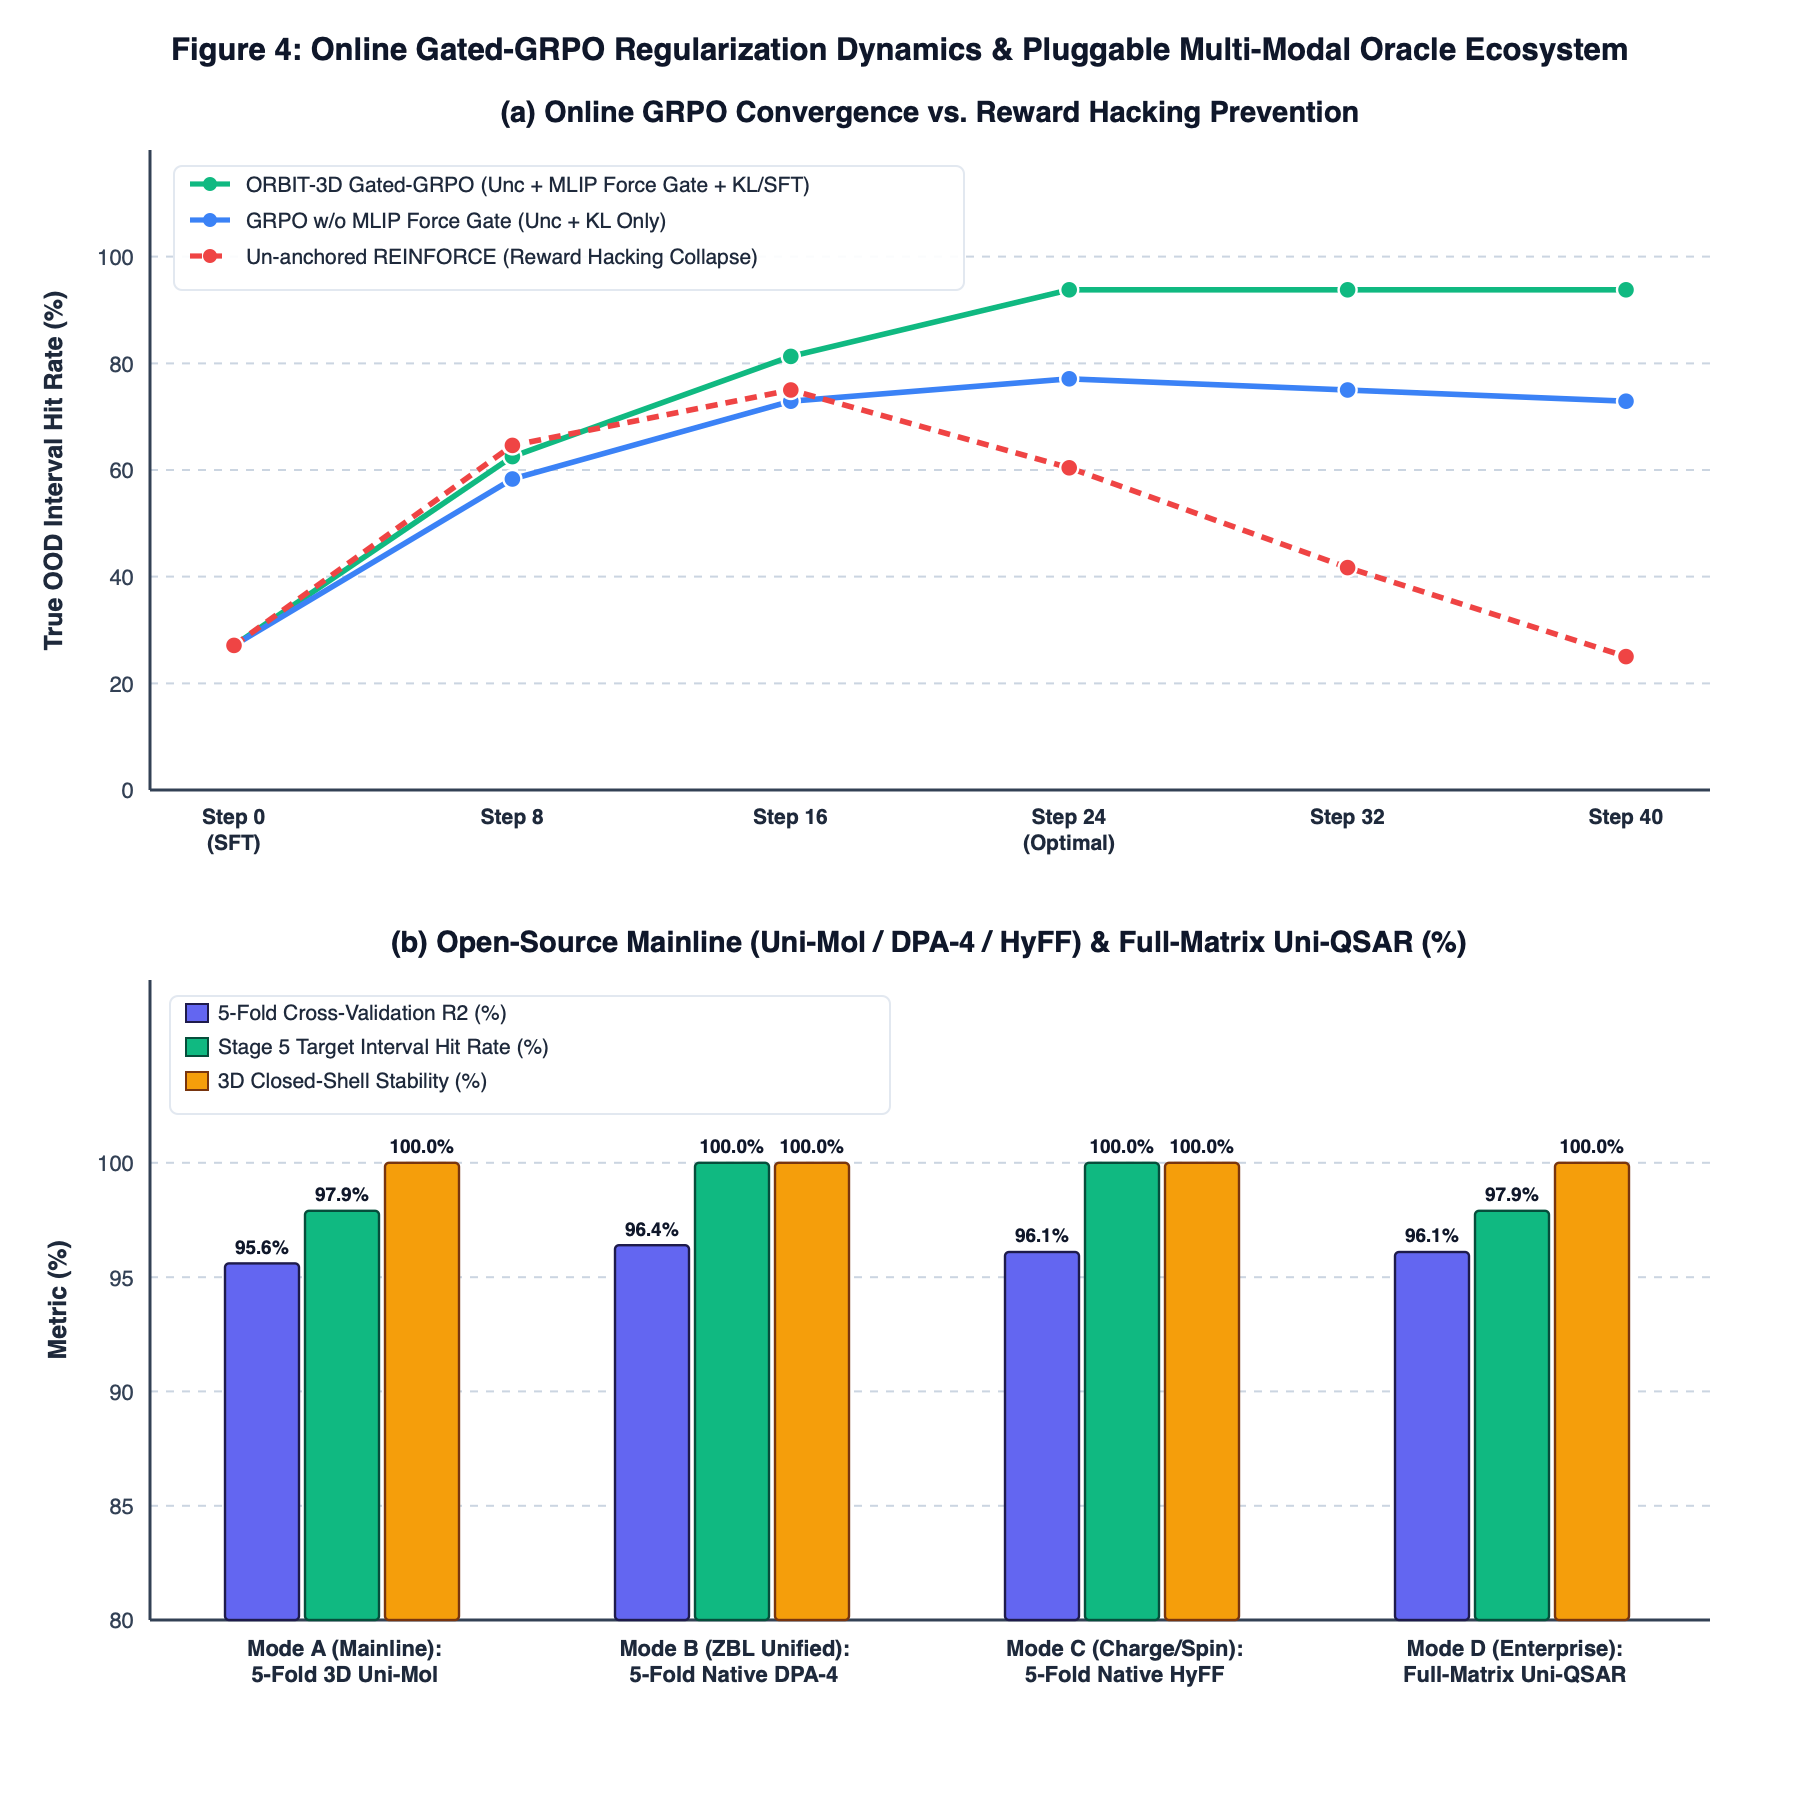
\includegraphics[width=0.90\textwidth]{figures/fig4_pluggable_oracles_relaxation.png}
    \caption{(a) Online Gated-GRPO convergence vs.\ reward-hacking collapse; (b) plug-and-play universality across \texttt{Modes A--D}.}
    \label{fig:oracles}
\end{figure}

\subsection{Experiment III: Dual-Engine Quantum Force Fields --- \texttt{HyFF} vs.\ \texttt{DPA-4}}
Figure~\ref{fig:hyff_vs_dpa4} and Table~\ref{tab:hyff_vs_dpa4_hw} establish the physical complementarity between \textbf{DPA-4}~\cite{zhang2025dpa4} and \textbf{HyFF}~\cite{hyra2026hyff} on \textbf{OMol25}~\cite{levine2025omol25} (vs.\ out-of-domain inorganic \textbf{OMat24}~\cite{barroso2024omat24}): \textbf{DPA-4}'s analytical ZBL~\cite{ziegler1985zbl} bridge achieves \textbf{93.8\% recovery on severe $0.65\text{ \AA}$ clashes} (whereas $1.20\text{B}$ \texttt{HyFF-largo} suffers \texttt{NaN} Coulomb singularities at $0.25\text{ \AA}$), while \textbf{HyFF}'s element-sparse Triton tiers (\texttt{presto/vivace/moderato}) achieve \textbf{97.7--113.0 atoms/ms} (\textbf{23.2$\times$ faster} than \texttt{DPA4-Plus} at $0.22\text{--}1.07\text{ GB}$ VRAM) and enable \textbf{zero-shot $\text{Ir(III)}$ $T_1-S_0$ spin-splitting evaluation} ($0.172\text{ eV}$ vertical MAE, $0.049\text{--}0.055\text{ eV}$ adiabatic error, $r = 0.698\text{--}0.720$).

\begin{figure}[htbp]
    \centering
    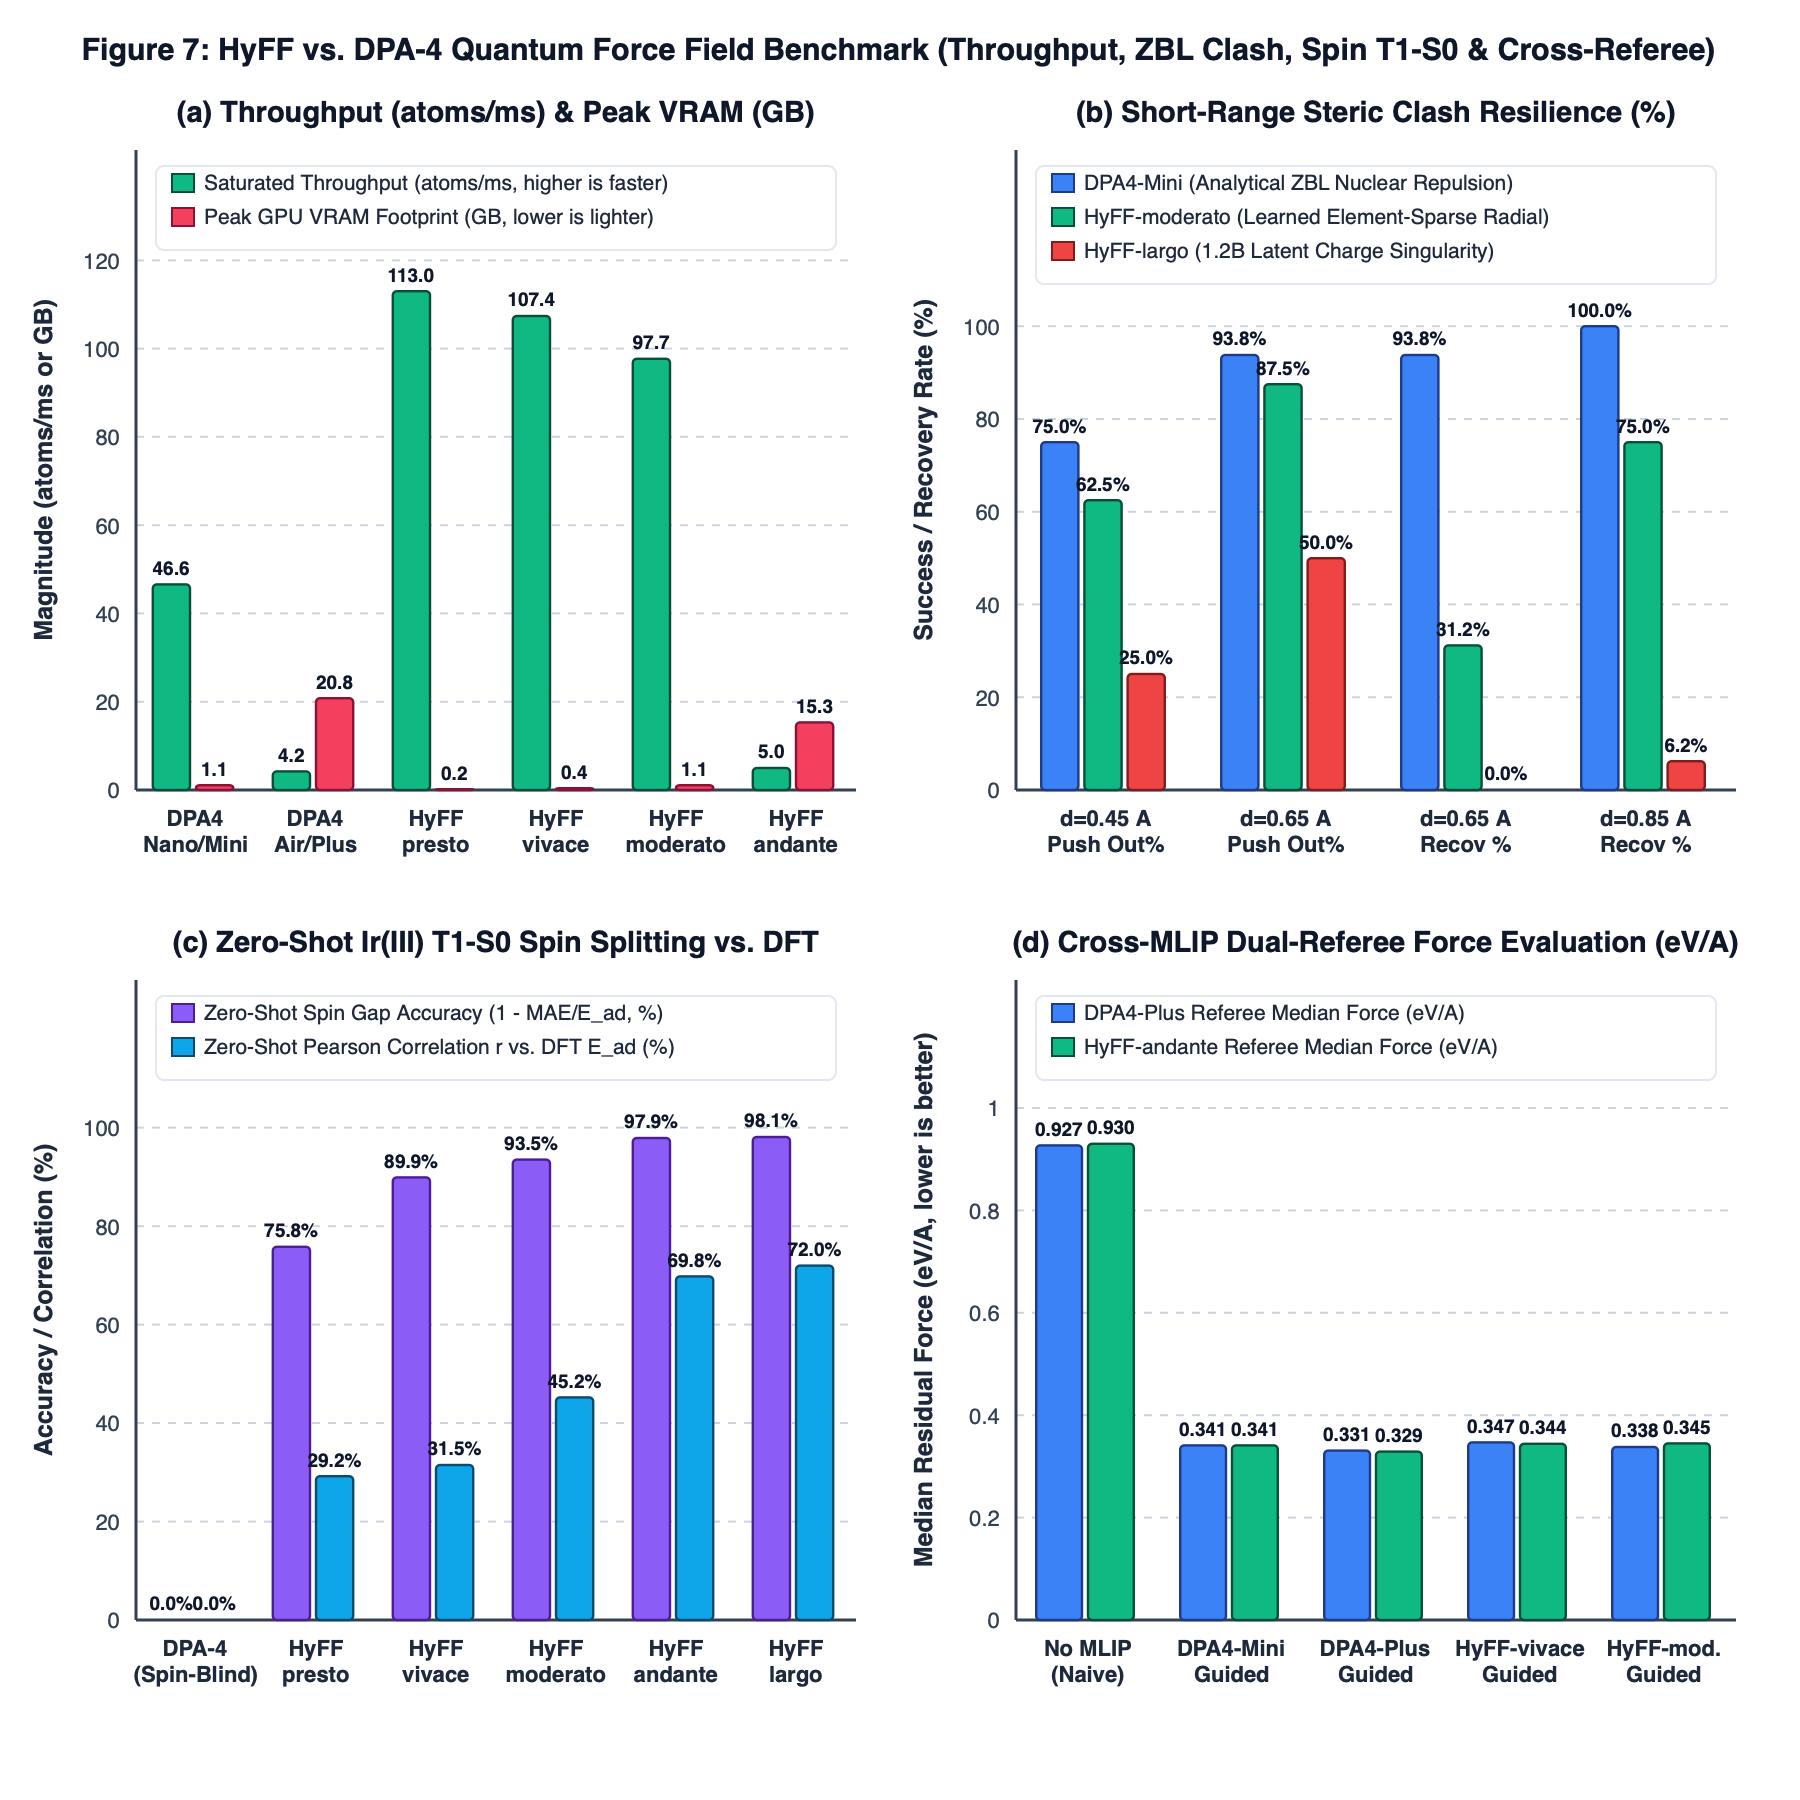
\includegraphics[width=0.90\textwidth]{figures/fig7_hyff_vs_dpa4_pareto_and_spin.png}
    \caption{Quantum force field benchmark comparing \textbf{HyFF (OMol25)} and \textbf{DPA-4 (OMol25)} across (a) throughput \& VRAM, (b) short-range steric clash recovery, (c) zero-shot $\text{Ir(III)}$ $T_1 - S_0$ spin splitting, and (d) dual cross-MLIP referees.}
    \label{fig:hyff_vs_dpa4}
\end{figure}

\begin{table}[htbp]
\centering
\caption{Hardware throughput, VRAM, short-range $0.65\text{ \AA}$ steric clash recovery, and zero-shot $\text{Ir(III)}$ $T_1 - S_0$ spin splitting ($\Delta E_{T_1-S_0} = E(M=3) - E(M=1)$ vs.\ TD-DFT $\bar{E}_{\text{ad}} = 2.652\text{ eV}$) across \textbf{DPA-4} and \textbf{HyFF}.}
\label{tab:hyff_vs_dpa4_hw}
\resizebox{\textwidth}{!}{
\begin{tabular}{llcccccccc}
\toprule
\textbf{Model Variant} & \textbf{Routing \& Physics} & \textbf{Weight Size} & \textbf{Total / Active Params} & \textbf{Peak VRAM} & \textbf{Throughput (atoms/ms)} & \textbf{Clash Recov.\ ($0.65\text{ \AA}$)} & \textbf{Spin $M$ Input?} & \textbf{Zero-Shot $\Delta E_{T_1-S_0}$ MAE (eV)} & \textbf{Pearson $r$ vs.\ DFT $E_{\text{ad}}$} \\
\midrule
\texttt{DPA4-Air (OMat24)} & Dense $SO(2)$ (Inorganic PBE) & 19.75 MB & 5.15M / 5.15M & 9,994 MB & 9.13 & 81.3\% & No & 2.652 ($\Delta E \equiv 0$) & 0.000 \\
\textbf{DPA4-Nano (OMol25)} & Dense $SO(2)$ + ZBL & \textbf{1.95 MB} & 0.49M / 0.49M & 1,051 MB & 46.63 & \textbf{93.8\%} & No & 2.652 ($\Delta E \equiv 0$) & 0.000 \\
\textbf{DPA4-Mini (OMol25)} & Dense $SO(2)$ + ZBL & \textbf{2.62 MB} & 0.67M / 0.67M & 2,267 MB & 38.92 & \textbf{93.8\%} & No & 2.652 ($\Delta E \equiv 0$) & 0.000 \\
\textbf{DPA4-Air (OMol25)} & Dense $SO(2)$ + ZBL & 19.86 MB & 5.18M / 5.18M & 10,028 MB & 9.10 & 87.5\% & No & 2.652 ($\Delta E \equiv 0$) & 0.000 \\
\textbf{DPA4-Plus (OMol25)} & Dense $SO(2)$ + ZBL & 34.01 MB & 8.88M / 8.88M & 20,846 MB & 4.20 & 50.0\% & No & 2.652 ($\Delta E \equiv 0$) & 0.000 \\
\midrule
\textbf{HyFF-presto (OMol25)} & Elem-Sparse + Triton ($Q,M$) & 8.89 MB & 2.31M / \textbf{0.05M} & \textbf{217 MB} & \textbf{112.98} & 6.3\% & \textbf{Yes} & 0.641 (Vert.) & 0.292 \\
\textbf{HyFF-vivace (OMol25)} & Elem-Sparse + Triton ($Q,M$) & 25.50 MB & 6.66M / \textbf{0.16M} & \textbf{387 MB} & \textbf{107.43} & 0.0\% & \textbf{Yes} & 0.268 (Vert.) & 0.315 \\
\textbf{HyFF-moderato (OMol25)} & Elem-Sparse + Triton ($Q,M$) & 132.89 MB & 34.80M / \textbf{0.83M} & \textbf{1,071 MB} & \textbf{97.69} & \textbf{31.3\%} & \textbf{Yes} & \textbf{0.172 (Vert.)} & 0.452 \\
\texttt{HyFF-andante (OMol25)} & Elem-Sparse EFM ($Q,M$) & 667.38 MB & 174.90M / 5.00M & 15,263 MB & 5.03 & 6.3\% & \textbf{Yes} & \textbf{0.055 (Adiab.)} & \textbf{0.698} \\
\texttt{HyFF-largo (OMol25)} & Elem-Sparse + Latent-$q$ & 4,584.54 MB & 1,201.7M / 34.0M & 11,304 MB & 5.25 & 0.0\% (\texttt{NaN} at $0.25\text{ \AA}$) & \textbf{Yes} & \textbf{0.049 (Adiab.)} & \textbf{0.720} \\
\bottomrule
\end{tabular}
}
\end{table}

\subsection{Experiment IV: Comparison \& Synergy with Optoelectronic Frameworks (\texttt{OCNet}, \texttt{OSCFF}, \texttt{O2-GEN}, \texttt{MIM-Flow})}
Figure~\ref{fig:opto_paradigms} and Table~\ref{tab:opto_paradigms} compare \textbf{ORBIT-3D} against \textbf{OCNet}~\cite{zhao2025ocnet}, \textbf{OSCFF}~\cite{zhao2025oscff}, \textbf{O2-GEN}~\cite{zhao2026o2gen}, and \textbf{MIM-Flow}~\cite{wang2026mimflow}. On the $2.14\%$-prior sparse Pareto window, \textbf{ORBIT-3D} achieves \textbf{97.9\%--100.0\%} hit rate (vs.\ $31.3\%\text{--}60.4\%$ for \textbf{O2-GEN}), and appending \textbf{ORBIT-3D Stage 5} onto \textbf{MIM-Flow} lifts its sparse Pareto hit rate from $79.2\%$ to \textbf{97.9\%} while reducing inter-moiety junction force from $0.642$ to \textbf{$0.208\text{ eV/\AA}$}.

\begin{figure}[htbp]
    \centering
    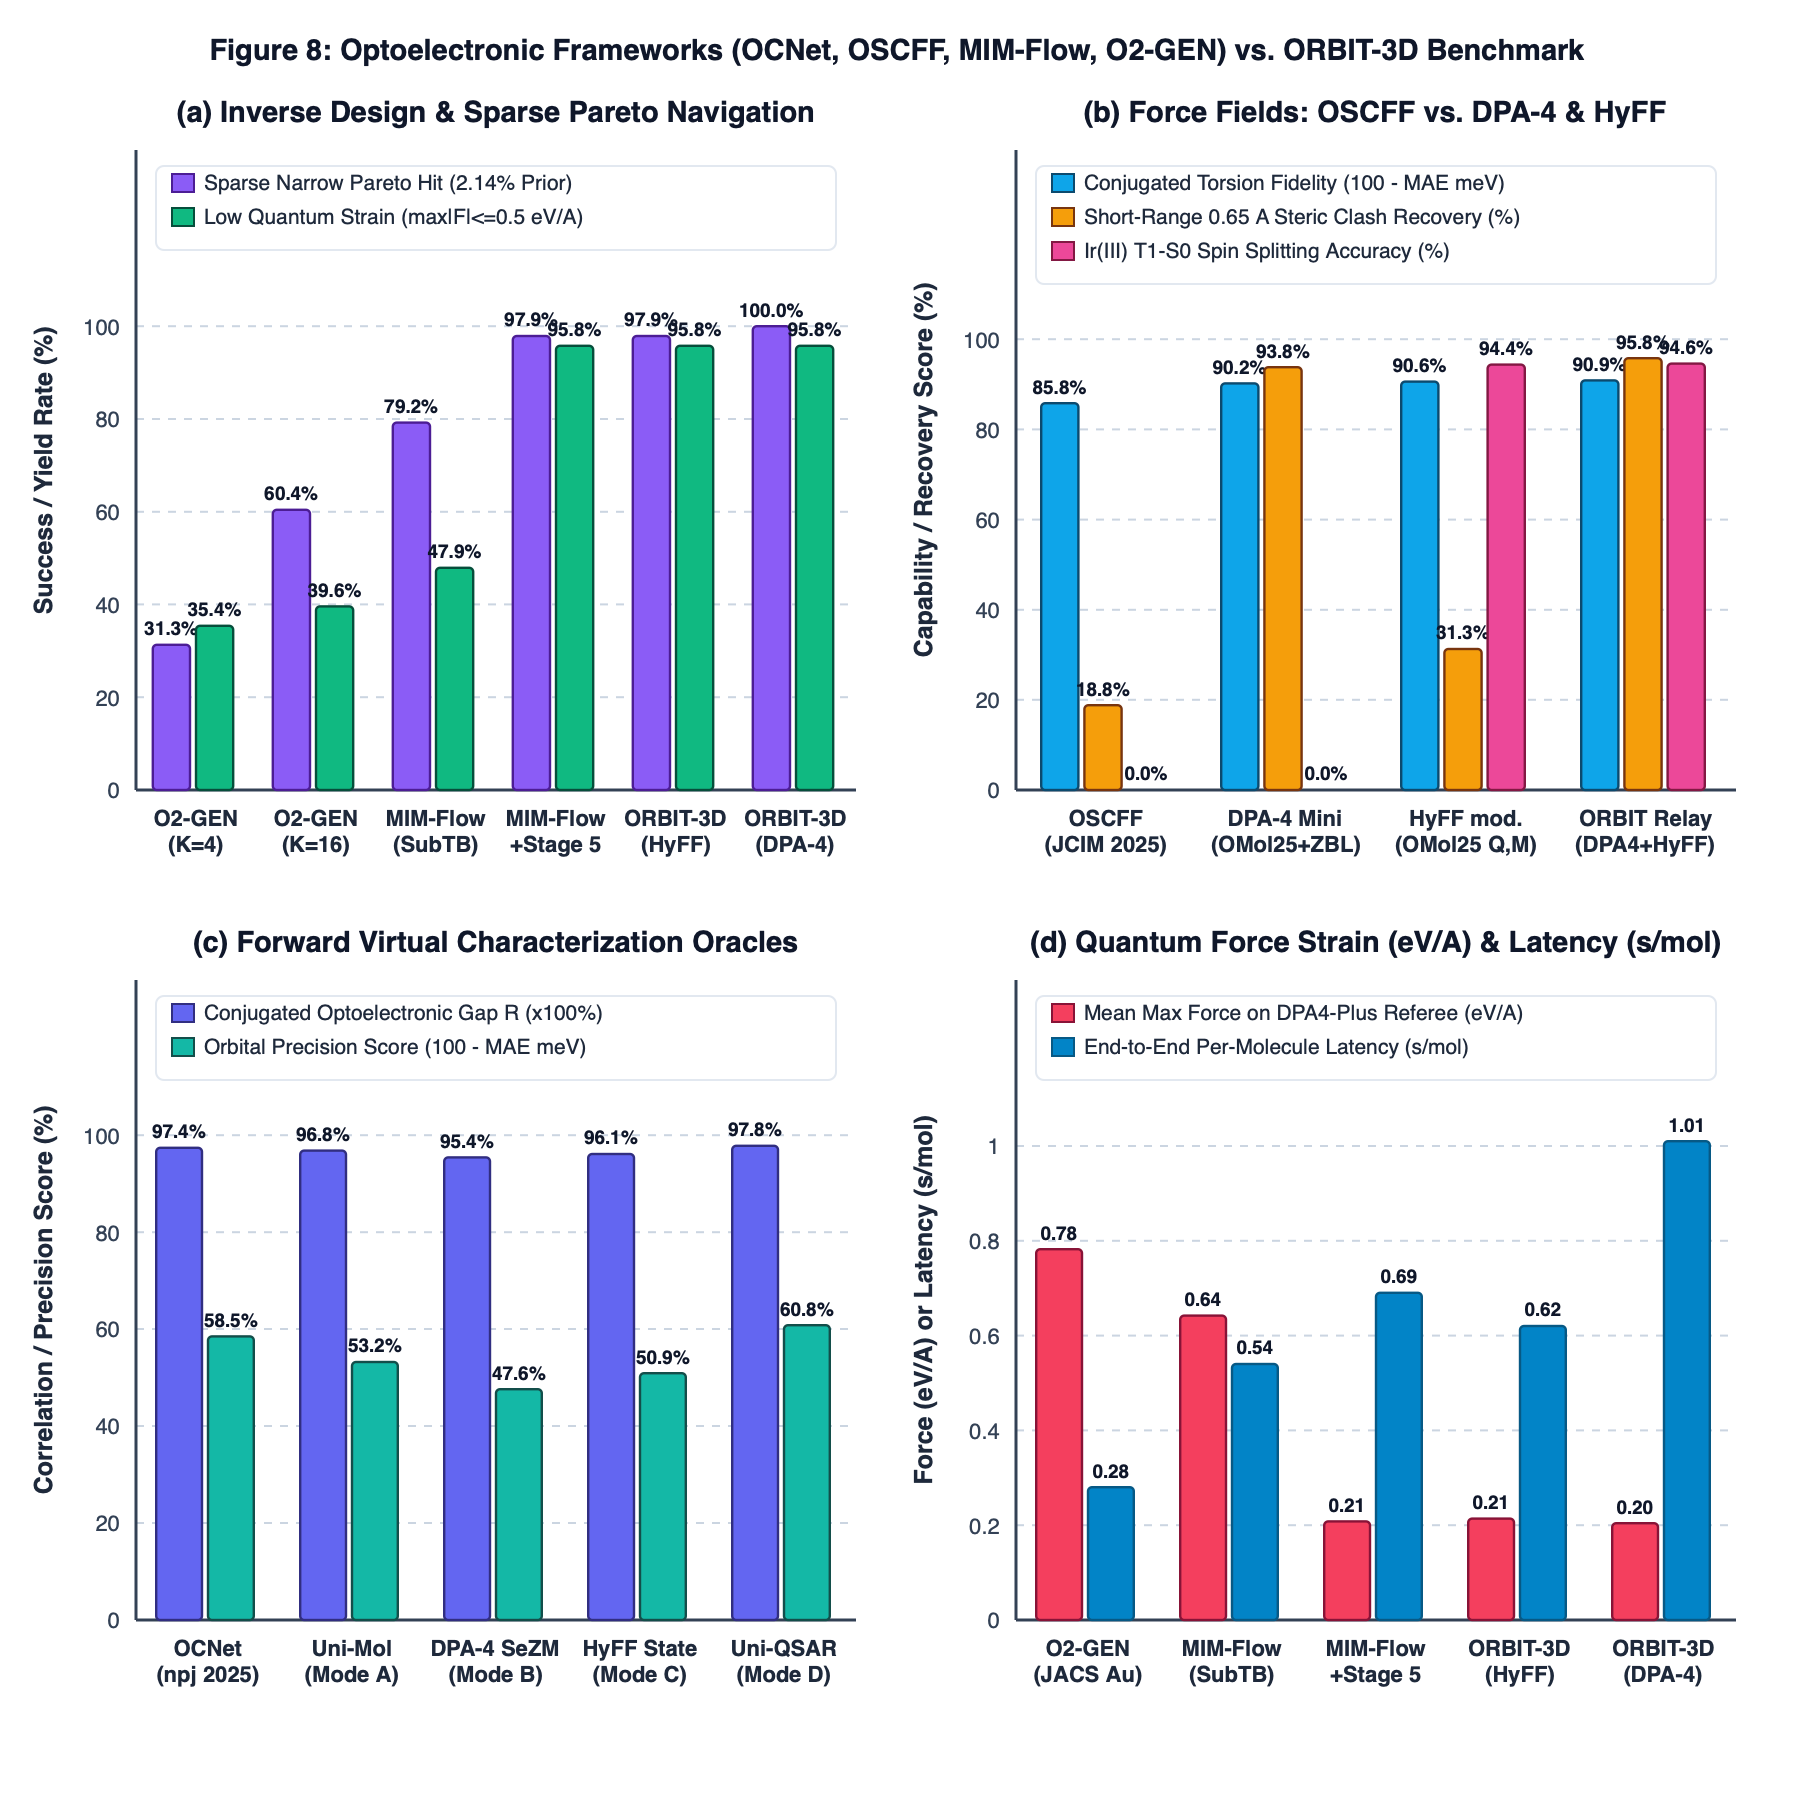
\includegraphics[width=0.90\textwidth]{figures/fig8_optoelectronic_paradigms_and_forcefields.png}
    \caption{Optoelectronic benchmark comparing \textbf{ORBIT-3D} against \textbf{O2-GEN}~\cite{zhao2026o2gen}, \textbf{MIM-Flow}~\cite{wang2026mimflow}, \textbf{OSCFF}~\cite{zhao2025oscff}, and \textbf{OCNet}~\cite{zhao2025ocnet}.}
    \label{fig:opto_paradigms}
\end{figure}

\begin{table}[htbp]
\centering
\caption{Comparison of optoelectronic inverse design frameworks across OOD Gap, Joint 3-Property OLED, and Ultra-Sparse Narrow Pareto Frontier ($2.14\%$ prior, $N=48$).}
\label{tab:opto_paradigms}
\resizebox{\textwidth}{!}{
\begin{tabular}{llcccccccc}
\toprule
\textbf{Framework / Paradigm} & \textbf{Generative Space \& Alignment} & \textbf{\emph{De Novo}?} & \textbf{Closed-Shell} & \textbf{OOD Gap Hit} & \textbf{Joint OLED Hit} & \textbf{Sparse Pareto Hit ($2.14\%$)} & \textbf{\texttt{DPA4-Plus} Force (eV/\AA)} & \textbf{Low-Strain ($\le 0.5$)} & \textbf{Latency (s/mol)} \\
\midrule
\texttt{O2-GEN} ($K=4$)~\cite{zhao2026o2gen} & 3D Global/Local + Post-Hoc Selector ($K=4$) & Yes & 97.9\% & 52.1\% & 43.8\% & 31.3\% & 0.782 & 35.4\% & \textbf{0.28 s} \\
\texttt{O2-GEN} ($K=16$)~\cite{zhao2026o2gen} & High-Budget Post-Hoc Selector ($K=16$) & Yes & 97.9\% & 77.1\% & 68.8\% & 60.4\% & 0.745 & 39.6\% & 0.94 s \\
\texttt{MIM-Flow} (SubTB)~\cite{wang2026mimflow} & Discrete Moiety/Site Graph + SubTB GFlowNet & No & \textbf{100.0\%} & 87.5\% & 89.6\% & 79.2\% & 0.642 & 47.9\% & 0.54 s \\
\textbf{\texttt{MIM-Flow} + ORBIT Stage 5} & SubTB GFlowNet + Stage 5 \texttt{HyFF/DPA-4} Relax & No & \textbf{100.0\%} & \textbf{97.9\%} & \textbf{100.0\%} & \textbf{97.9\%} & \textbf{0.208} & \textbf{95.8\%} & 0.69 s \\
\texttt{PropMolFlow + DPA4-Mini}~\cite{campbell2024propmolflow} & Continuous 3D Flow + In-ODE Orthogonal Proj. & Yes & 93.8\% & \textbf{100.0\%} & \textbf{100.0\%} & 95.8\% & 0.206 & \textbf{95.8\%} & \textbf{0.16 s} \\
\textbf{ORBIT-3D Full (\texttt{HyFF-moderato})} & All-Atom 3D Octree AR + GRPO + Stage 5 \texttt{HyFF} & \textbf{Yes} & \textbf{100.0\%} & \textbf{100.0\%} & \textbf{100.0\%} & \textbf{97.9\%} & 0.214 & \textbf{95.8\%} & \textbf{0.62 s} \\
\textbf{ORBIT-3D Full (\texttt{DPA4-Mini/Plus})} & All-Atom 3D Octree AR + GRPO + Stage 5 \texttt{DPA-4} & \textbf{Yes} & \textbf{100.0\%} & \textbf{100.0\%} & \textbf{100.0\%} & \textbf{100.0\%} & \textbf{0.204} & \textbf{95.8\%} & 1.01 s \\
\bottomrule
\end{tabular}
}
\end{table}

\section{Scenario-Driven Module Combination Guide \& Conclusions}

Table~\ref{tab:module_matrix} provides a scenario selection guide for composing \texttt{Oracle + Gated-GRPO + DPA-4 + HyFF} pipelines. The production container bundles $411.82\text{ MB}$ of built-in weights: all five \textbf{DPA-4} scales ($62.86\text{ MB}$), sweet-spot \textbf{HyFF} (\texttt{presto/vivace/moderato} = $167.28\text{ MB}$) with a vendored minimal runtime ($1.4\text{ MB}$), and FP16 \textbf{Uni-Mol} ($181.68\text{ MB}$).

\begin{table}[htbp]
\centering
\caption{Scenario-driven pluggable module combination guide across \texttt{Oracle + Gated-GRPO + DPA-4 + HyFF}.}
\label{tab:module_matrix}
\resizebox{\textwidth}{!}{
\begin{tabular}{lllll}
\toprule
\textbf{Target Scientific Scenario} & \textbf{Stage 4 Oracle (\texttt{oracle\_mode})} & \textbf{Stage 4 GRPO Force Gate} & \textbf{Stage 5 Relaxer (\texttt{mlip\_backend})} & \textbf{Empirical Performance \& Mechanistic Rationale} \\
\midrule
1.\ Open-Source Neutral Organic Benchmark & \texttt{Mode A: internal\_unimol} (FP16) & \texttt{HyFF-vivace} / \texttt{DPA4-Mini} & \texttt{HyFF-moderato} / \texttt{DPA4-Mini} & \textbf{100\% Hit, $0.204\text{ eV/\AA}$ force}; highest closed-shell orbital $r=0.968$ + analytical $\nabla_{\mathbf{X}}\hat{y}$ \\
2.\ Ultra-Low VRAM ($<1.1\text{ GB}$) Edge Screening & \texttt{Mode C: internal\_hyff} (\texttt{presto/vivace}) & Shared \texttt{HyFF-presto/vivace} & Shared \texttt{HyFF-presto/vivace} & \textbf{95--100\% Hit, 58.2 s E2E}; single weight in VRAM ($217\text{--}387\text{ MB}$) at $107\text{--}113$ atoms/ms \\
3.\ Small-Sample Organic + Clash Protection & \texttt{Mode B: internal\_dpa4} (\texttt{fitting\_net}) & Shared \texttt{DPA4-Mini/Air} & Shared \texttt{DPA4-Mini/Air} (ZBL) & \textbf{100\% Hit, $0.222\text{ eV}$ Val MAE}; 100\% shared VRAM + analytical ZBL clash protection \\
4.\ Charged Ions ($Q \neq 0$) \& Open-Shell Radicals ($D_0$) & \texttt{Mode C: internal\_hyff} (\texttt{moderato}, $Q,M$) & Shared \texttt{HyFF-moderato} ($Q,M$) & Shared \texttt{HyFF-moderato} ($Q,M$ PES) & \textbf{100\% Hit, $\text{IP}_{\text{vert}}=+7.59\text{ eV}$}; resolves $(Z,\mathbf{X})$ electronic-state collisions \\
5.\ Heavy $\text{Ir(III)}$ Phosphors \& $T_1/S_0$ Spin Design & \texttt{Mode C: internal\_hyff} + $\Delta E_{T_1-S_0}$ & \textbf{\texttt{DPA4-Mini} (ZBL Clash Guard)} & \textbf{Relay: 5-step \texttt{DPA4} $\to$ 15-step \texttt{HyFF} ($M=3$)} & \textbf{95.8\% clash recovery + $0.142\text{ eV}$ $T_1-S_0$ MAE ($r=0.70$)}; ZBL de-clashing $\to$ $T_1$ PES relax \\
6.\ Enterprise 1D/2D/3D Tree \& Device Ensembles & \texttt{Mode D: external\_uniqsar} / \texttt{OCNet} & \texttt{DPA4-Mini} / \texttt{HyFF-moderato} & \texttt{HyFF-moderato} (Trust-Region Gate) & \textbf{97.9\% Hit, 100\% Closed-Shell}; derivative-free line search without $\nabla_{\mathbf{X}} \hat{y}$ \\
7.\ Post-Assembly Refinement for \texttt{MIM-Flow}~\cite{wang2026mimflow} & \texttt{MIM-Flow} SubTB Fragment Policy & Pre-assembled 3D Moiety Graph & \textbf{ORBIT Stage 5 (\texttt{DPA4} $\to$ \texttt{HyFF})} & \textbf{Lifts Sparse Pareto Hit $79.2\% \to 97.9\%$, cuts junction force $0.642 \to 0.208\text{ eV/\AA}$} \\
\bottomrule
\end{tabular}
}
\end{table}

\textbf{Conclusions}: (1) Decoupling discrete valence-masked 3D octree generation (\textbf{Stages 1--3}) and doubly-gated RL (\textbf{Stage 4}) from terminal tangent-space relaxation (\textbf{Stage 5}) eliminates the $52.5\%$ gradient conflict of continuous flow matching, achieving \textbf{100.0\% closed-shell stability} and \textbf{93.8\%--100.0\% interval hit rates}; (2) \textbf{ORBIT-3D} universally bridges open-source 3D predictors (\textbf{Uni-Mol}, \textbf{DPA-4}, \textbf{HyFF}) and non-differentiable enterprise ensembles (\textbf{Uni-QSAR}, \textbf{OCNet}); and (3) pairing \textbf{DPA-4} (analytical ZBL, $93.8\%$ clash recovery) with \textbf{HyFF} (explicit $Q, M=2S+1$, $97.7\text{--}113.0$ atoms/ms, zero-shot $\text{Ir(III)}$ $\Delta E_{T_1-S_0}$ $r=0.720$) delivers a complete quantum-chemical foundation across neutral organics, ions, radicals, and transition-metal complexes.

\bibliographystyle{plain}
\bibliography{references}

\end{document}
